\documentclass[addpoints,a4paper]{exam}

\usepackage{amsmath, amsfonts, amssymb, amsthm}
\usepackage{booktabs}
\usepackage{enumitem}
\usepackage{graphicx}
\usepackage{multirow}
\usepackage{tabularx}
\usepackage{pythonhighlight}

\printanswers

\begin{document}
\begin{flushleft}
  { \large \textsf{\textbf{Spring 2022, CS 412: Algorithms: Design and Analysis,  Quiz 6 -- L3}}}\vspace{.5em}

  Friday, 29 April, 2022. Total Marks: \numpoints, Duration: 20 minutes.
\end{flushleft}

{\bf Instructions:}

\begin{enumerate}
  % \item Please observe the allowed time for this quiz as indicated on Canvas.
\item Solve the problems by hand on blank A4 paper in clear and legible handwriting.
\item Work in pencil will be considered rough work and will not be graded.
  % \item You may consult external resources, e.g. the book or the internet. However, we trust that you will not use this access to collaborate with other people (directly or through forums) on the problems.
  % \item For each question, justify your answer. Simply stating the answer will not be sufficient.
\item Include the following header string on each sheet that you work on: \texttt{<name>, <section>, <ID>, Quiz 5}. For example, \texttt{Cheeti Khan, L1, ck00042, Quiz 5}.
  % \item Submission is on Canvas in the form of scans / photographs of your work in a single PDF file. Please ensure good lighting and readability in the scans / photographs and that the header string is clearly visible on each page. We cannot grade what we cannot read or what we cannot verify as your work.
  % \item Rename the file to \texttt{<ID>-<section>.pdf}, e.g. \texttt{ck00042-L1.pdf} before uploading.
\end{enumerate}
\centerline{\rule{.7\textwidth}{1pt}}

\begin{questions}
\question The problem is described below. The description requires to read input and print the output. Instead, you have to write a single function, \pyth{solve}, in a file, \texttt{solve.py}, that takes the input as argument and returns the desired output as a \pyth{list} of numbers.
  
\noindent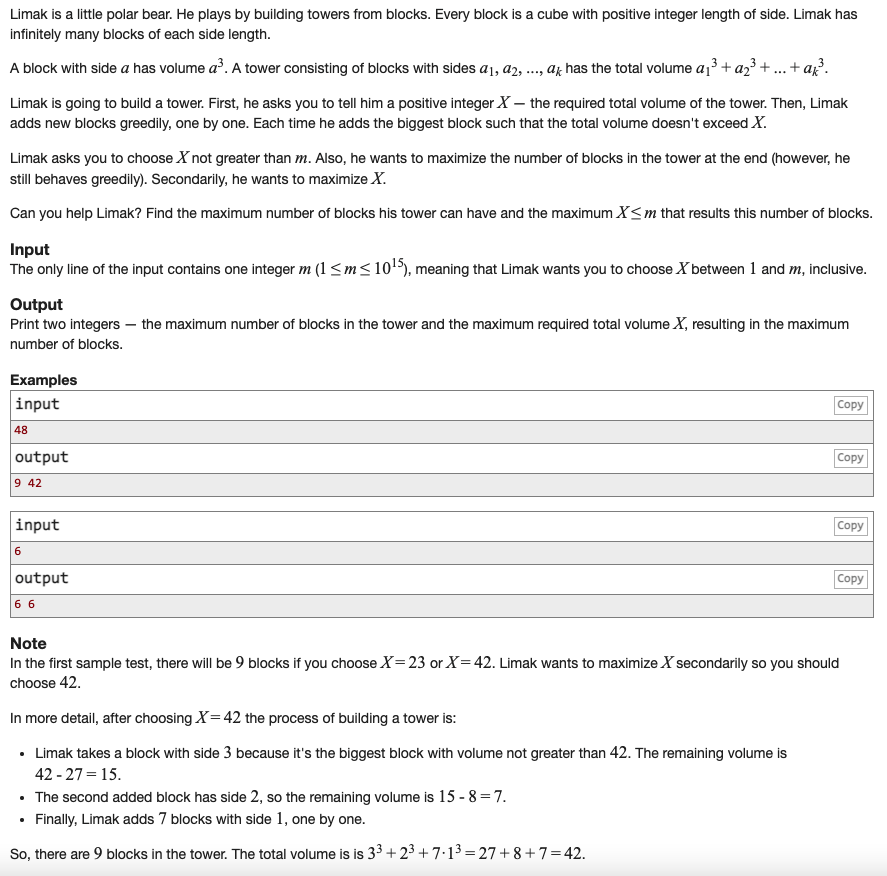
\includegraphics[width=\textwidth]{problem}
\centerline{\rule{.3\textwidth}{1pt}viel Gl\"uck\rule{.3\textwidth}{1pt}}
\end{questions}
  

\end{document}

%%% Local Variables:
%%% mode: latex
%%% TeX-master: t
%%% End:
